\chapter[Agreement, odds ratio and relative risk]{Agreement, odds ratio\\ and relative risk}


\section{Measure agreement (kappa)}
Two people (MN és VU) qualified psychiatric patients. Do  they agree? 

\noindent\textbf{Calculate the $\kappa$ (kappa)  statistics and interpret the reults!}

\begin{flushright}
\small Source:
Wongpakaran et al.: A comparison of Cohen’s Kappa and Gwet’s AC1 when calculating inter-rater reliability coefficients: a study conducted with personality disorder samples,  BMC Research Methodolgy 2013,13:61. \\
\url{http://www.biomedcentral.com/1471-2288/13/61}
\end{flushright}




\begin{minipage}{0.5\textwidth}
	\subsection{Avoidant} 
	$\kappa=$\rule{2cm}{0.4pt}\quad agreement: \rule{2cm}{0.4pt}

	\subsection{Dependent}
	$p_o=0.9474$, $p_e=0.8532$\medskip
	
	$\kappa=$\rule{2cm}{0.4pt}\quad agreement: \rule{2cm}{0.4pt}
	\subsection{Depressive}
	$p_o=0.8947$, $p_e=0.7431$\medskip
		
		$\kappa=$\rule{2cm}{0.4pt}\quad agreement: \rule{2cm}{0.4pt}
	\subsection{Schizoid}
	$p_o=0.8421$, $p_e=0.6371$\medskip
		
		$\kappa=$\rule{2cm}{0.4pt}\quad agreement: \rule{2cm}{0.4pt}
	\subsection{Total antisocial} 
	$p_o=0.8947$, $p_e=0.8116$\medskip
		
		$\kappa=$\rule{2cm}{0.4pt}\quad agreement: \rule{2cm}{0.4pt}
\end{minipage}	
\hfill
\begin{minipage}{0.4\textwidth}
	
	\begin{tabular}{lc|cc}
	\toprule
	%\textbf{PDs}
					& 			& \multicolumn{2}{c}{\textbf{Rater VU}} 	\\
					& \textbf{Rater MN}	& NO & YES\\
					\midrule
	Avoidant 		& NO		& 14 & 0\\
					& YES		& 0  & 5\\
					\midrule
	Dependent 		& NO		& 17 & 1\\
					& YES		& 0  & 1\\
				\midrule
	Depressive 		& NO		& 15 & 1\\
					& YES		& 1  & 2\\
				\midrule
	Schizoid 		& NO		& 13 & 2\\
					& YES		& 1  & 3\\
				\midrule
	Total  			& NO		& 16 & 1\\
	antisocial		& YES		& 1  & 1\\
					\bottomrule
	\end{tabular}

\end{minipage}

\clearpage
\section{Odds ratio (OR)}
Children's drug use and risk factors were examined in a retrospective (case-control) study. Examine and interpret the odds ratios in the following table and determine the significance based on the confidence intervals
%Egy vizsgálatban a gyermekek droghasználatát és annak rizikótényezőit vizsgálták retrospektív (eset-kontroll) vizsgálatban Az alábbi táblázat adatai alapján ellenőrizze az esélyhányadosokat, értelmezze őket és állapítsa meg a szignifikanciát a confidence interval alapján!


\begin{center}
	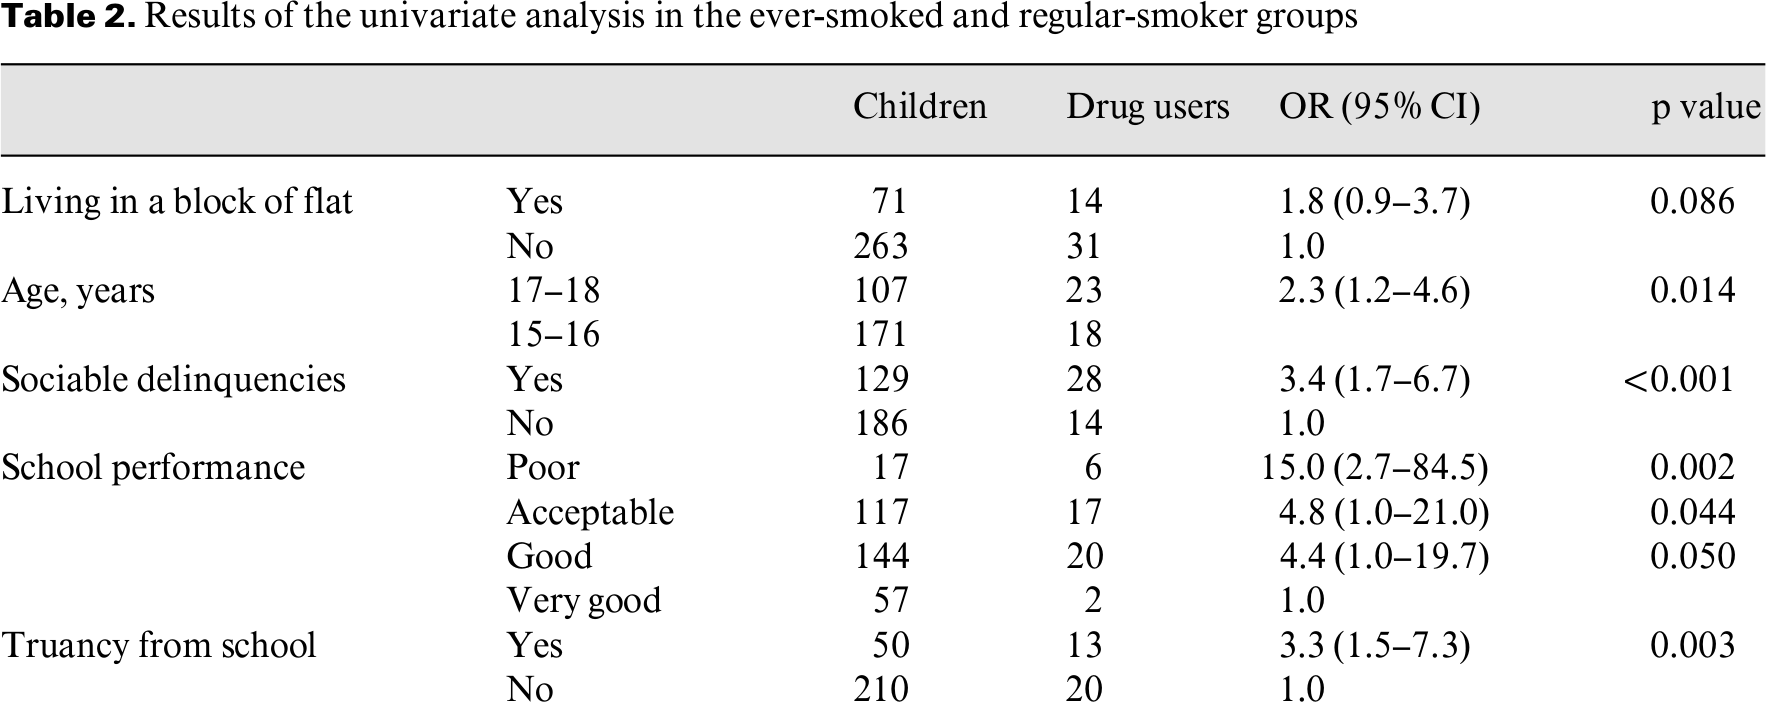
\includegraphics[width=0.9\textwidth]{G08-euraddict_table}
\end{center}


\begin{flushright}
\small Source: Nyári T.A., Herédi K. and Parker L.: Addictive Behaviour of Adolescents in Secondary Schools in Hungary.\\
	 Eur Addict Res 2005;11:38– 3 DOI:10.1159/00008141
\end{flushright}
Why did they calculate OR? \hrulefill


\subsection{Living in a block flat vs drug usage}
Table interpretation: in first row one can see that 14 children out 71 use drugs. In the second row 31 use druges out of 263. Create a 2$\times 2$ table and calculate the OR.
%az első sorban látható, hogy 71 gyerek közül 14 drogozik, a második sorban 263 gyerekből 31. Készítse el a 2x2-es táblázatot és számítsa ki az esélyhányadost (OR).

\begin{center}
		\begin{tabular}{r|C{15mm}C{15mm}|c}
		\toprule
			&\multicolumn{2}{c|}{\textbf{DRUG}}\\
		\textbf{Block flat}	&\textbf{yes}	&\textbf{no}	&Total\\
		\midrule
		\textbf{yes}	&	& &71\\		
		\textbf{no}	&	& &263\\
	%	\midrule
	%	Total			&	&	&\\
		\bottomrule
		\end{tabular}
\end{center}

\begin{enumerate}[a)]
\item The probability child use drug is
	\begin{itemize}
	\item when lives in block flat:  \rule{5cm}{0.4pt}
	\item when does not live in block flat: \rule{5cm}{0.4pt}
	\end{itemize}

\item  Quotient (OR)= \hrulefill

	Using the formula: \hrulefill

	Interpretation: \hrulefill
\item 95\% confidence interval: 	\hrulefill

\subsubsection*{Significance of odds ratio}
	\item H$_0$: \textsc{	\hrulefill}

			 H$_A$: \hrulefill
	\item Decision about significance based on CI: \hrulefill

	Decision based on $p$-value:	\hrulefill
\end{enumerate}

\subsection[School performance]{School performance. Compare the good and very good category with the drug usage. Calculate OR!}

\begin{center}
		\begin{tabular}{r|C{15mm}C{15mm}|c}
		\toprule
		\textbf{SCHOOL}		&\multicolumn{2}{c|}{\textbf{DRUG}}\\
		\textbf{PERFORMANCE}	&\textbf{yes}	&\textbf{no}	&Total\\	
		\midrule
		\textbf{good}	&	& &\\		
		\textbf{very good}	&	& &\\
	%	\midrule
	%	Total			&	&	&\\
		\bottomrule
		\end{tabular}
\end{center}

\begin{enumerate}[a)]

\item The probability that a child use drug if s/he is 
	\begin{itemize}
	\item good:  \rule{5cm}{0.4pt}
	\item very good: \rule{3.8cm}{0.4pt}
	\end{itemize}


\item  Quotient (OR)= \hrulefill

	Using the formula: \hrulefill

	Interpretation: \hrulefill
\item 95\% confidence interval: 	\hrulefill

\subsubsection*{Significance of odds ratio}
	\item H$_0$: \textsc{	\hrulefill}

			 H$_A$: \hrulefill
	\item Decision about significance based on CI: \hrulefill

	Decision based on $p$-value:	\hrulefill
\end{enumerate}

\subsection[Truancy]{Truancy from school and drug usage
Create 2$\times$2-es table and calculate OR.}

\begin{center}
		\begin{tabular}{r|C{15mm}C{15mm}|c}
		\toprule
			&\multicolumn{2}{c|}{\textbf{DRUG}}\\
		\textbf{TRUANCY}	&\textbf{yes}	&\textbf{no}	&Total\\
		\midrule
		\textbf{yes}	&	& &\\		
		\textbf{no}	&	& &\\
%		\midrule
%		Total			&	&	&\\
		\bottomrule
		\end{tabular}
\end{center}

\begin{enumerate}[a)]
\item The probability that a child use drug if he 
	\begin{itemize}
	\item plays truant:  \rule{5cm}{0.4pt}
	\item does not play truant: \rule{4.2cm}{0.4pt}
	\end{itemize}


\item  Quotient (OR)= \hrulefill

	Using the formula: \hrulefill

	Interpretation: \hrulefill
\item 95\% confidence interval: 	\hrulefill

\subsubsection*{Significance of odds ratio}
	\item H$_0$: \textsc{	\hrulefill}

			 H$_A$: \hrulefill
	\item Decision about significance based on CI: \hrulefill

	Decision based on $p$-value:	\hrulefill
\end{enumerate}




\section{Relative risk (RR)}
In a prospective study risks of respiratory complications were examined.% Examine the relative risks and $p$-values
%Egy prospektív vizsgálatban gyermekek altatása során fellépő kockázati tényezők rizikófaktorait vizsgálták. Ellenőrizzük a táblázat alapján a kapott relatív kockázatokat és $p$-értékeket!


\begin{center}
	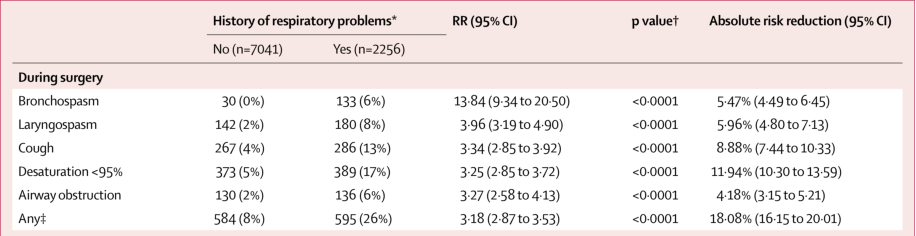
\includegraphics[width=\textwidth]{G08-RR_cikk_tabla}
\end{center}
\begin{flushright}
\small
Source: Britta S von Ungern-Sternberg és mtsai: Risk assessment for respiratory complications in paediatricanaesthesia:
a prospective cohort study. The Lancet, Vol 376 September 4, 2010, 773-783
\end{flushright}

\noindent Why did they calculate relative risk? \hrulefill\bigskip



\noindent\textbf{Examine using the table whether a respiratory problems (=yes) causes  more frequent brochospasmus complication!
Calculate a 2$\times$2-es táble and RR!}

\begin{center}
		\begin{tabular}{r|C{15mm}C{15mm}|c}
		\toprule
		\textbf{RESPIRATORY}	&\multicolumn{2}{c|}{\textbf{COMPLICATION}}\\
		\textbf{PROBLEMS}			&\textbf{yes}	&\textbf{no}	&Total\\
		\midrule
		\textbf{yes}	& 133	& & 2256\\		
		\textbf{no}	& 30	& & 7041\\
	%	\midrule
	%	Total		&		& &\\
		\bottomrule
		\end{tabular}
\end{center}


\begin{enumerate}[a)]
\item The risk of having complication if patient 
	\begin{itemize}
	\item had respiratory problems before: \rule{5cm}{0.4pt}
	\item did not have respiratory problems before: \rule{4.2cm}{0.4pt}
	\end{itemize}

\item Quotient (RR)= \hrulefill

	 Using the formula: \hrulefill

	Interpretation: 	\hrulefill
\item 95\% confidence interval of the relative risk: 	\hrulefill

\subsubsection*{Significance of the relative risk}
	\item H$_0$: \textsc{	\hrulefill}

		H$_A$: \hrulefill
	\item Decision about significance based on CI: \hrulefill

	Decision based on $p$-value:	\hrulefill
\end{enumerate}


